\chapter{SPECIFICAȚII ȘI REPREZENTAREA APLICAȚIEI}
Aplicația Fast Ride este construită folosind o arhitectură scalabilă, bazată pe microservicii și servicii în cloud. Tehnologiile principale utilizate sunt Blazor WebAssembly pentru interfața utilizator și Azure Durable Functions pentru logica de backend. Comunicarea dintre cele două componente este realizată prin API-uri HTTP și prin WebSocket-uri cu ajutorul SignalR.
\begin{figure}[H]
    \centering
    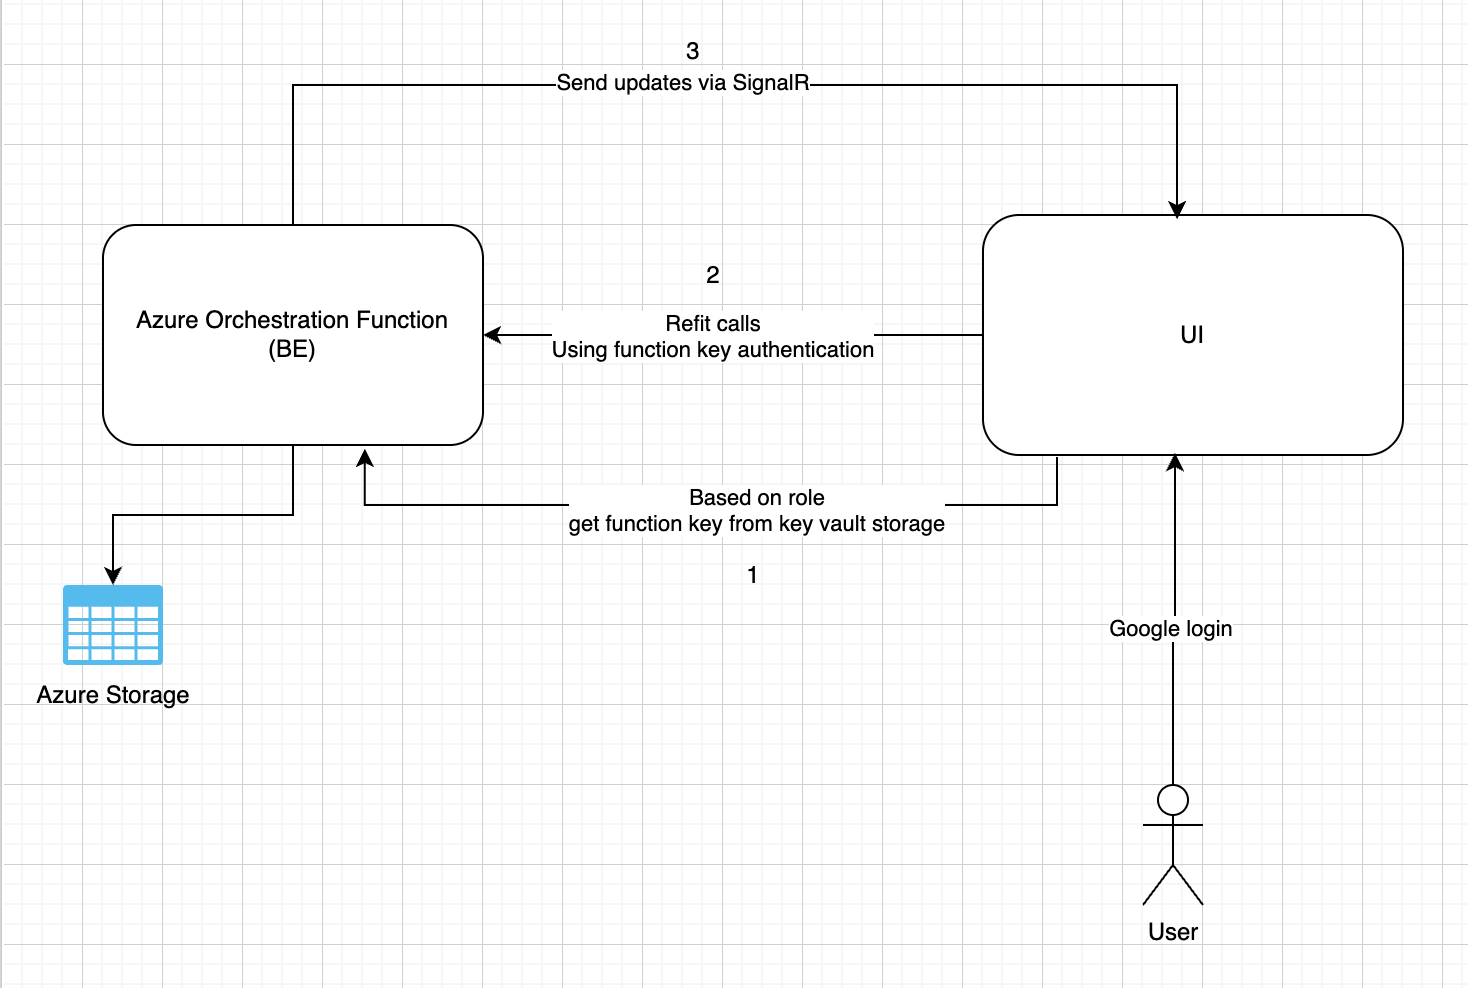
\includegraphics[width=14cm]{Assets/componentsComunication.png}
    \caption{Comunicarea dintre componentele proiectului}
    \label{fig:componentsComunication}
\end{figure}

\section{Arhitectura aplicației}
Aplicația dispunde de trei nivele:
\begin{itemize}
    \item stocare - unde se păstrează informațiile
    \item server-side - unde se prelucrează toate infomațiile
    \item client-side - unde se afisează toate informațiile către utilizatori
\end{itemize}

\subsection{Stocare}

Azure Table Storage este o bază de date NoSQL, ideală pentru scenarii în care se lucrează cu volume mari de date structurate,
dar fără relații complexe între entități. În cazul aplicației FastRide, fiecare entitate: utilizatori, curse, șoferi online și instanțele de orchestrare, este reprezentată ca o tabelă separată în Table Storage. Fiecare înregistrare (sau entitate) dintr-o tabelă este identificată în mod unic printr-o combinație de \textit{PartitionKey} și \textit{RowKey}, ceea ce asigură o distribuire eficientă și acces rapid la date.
\begin{figure}[H]
    \centering
    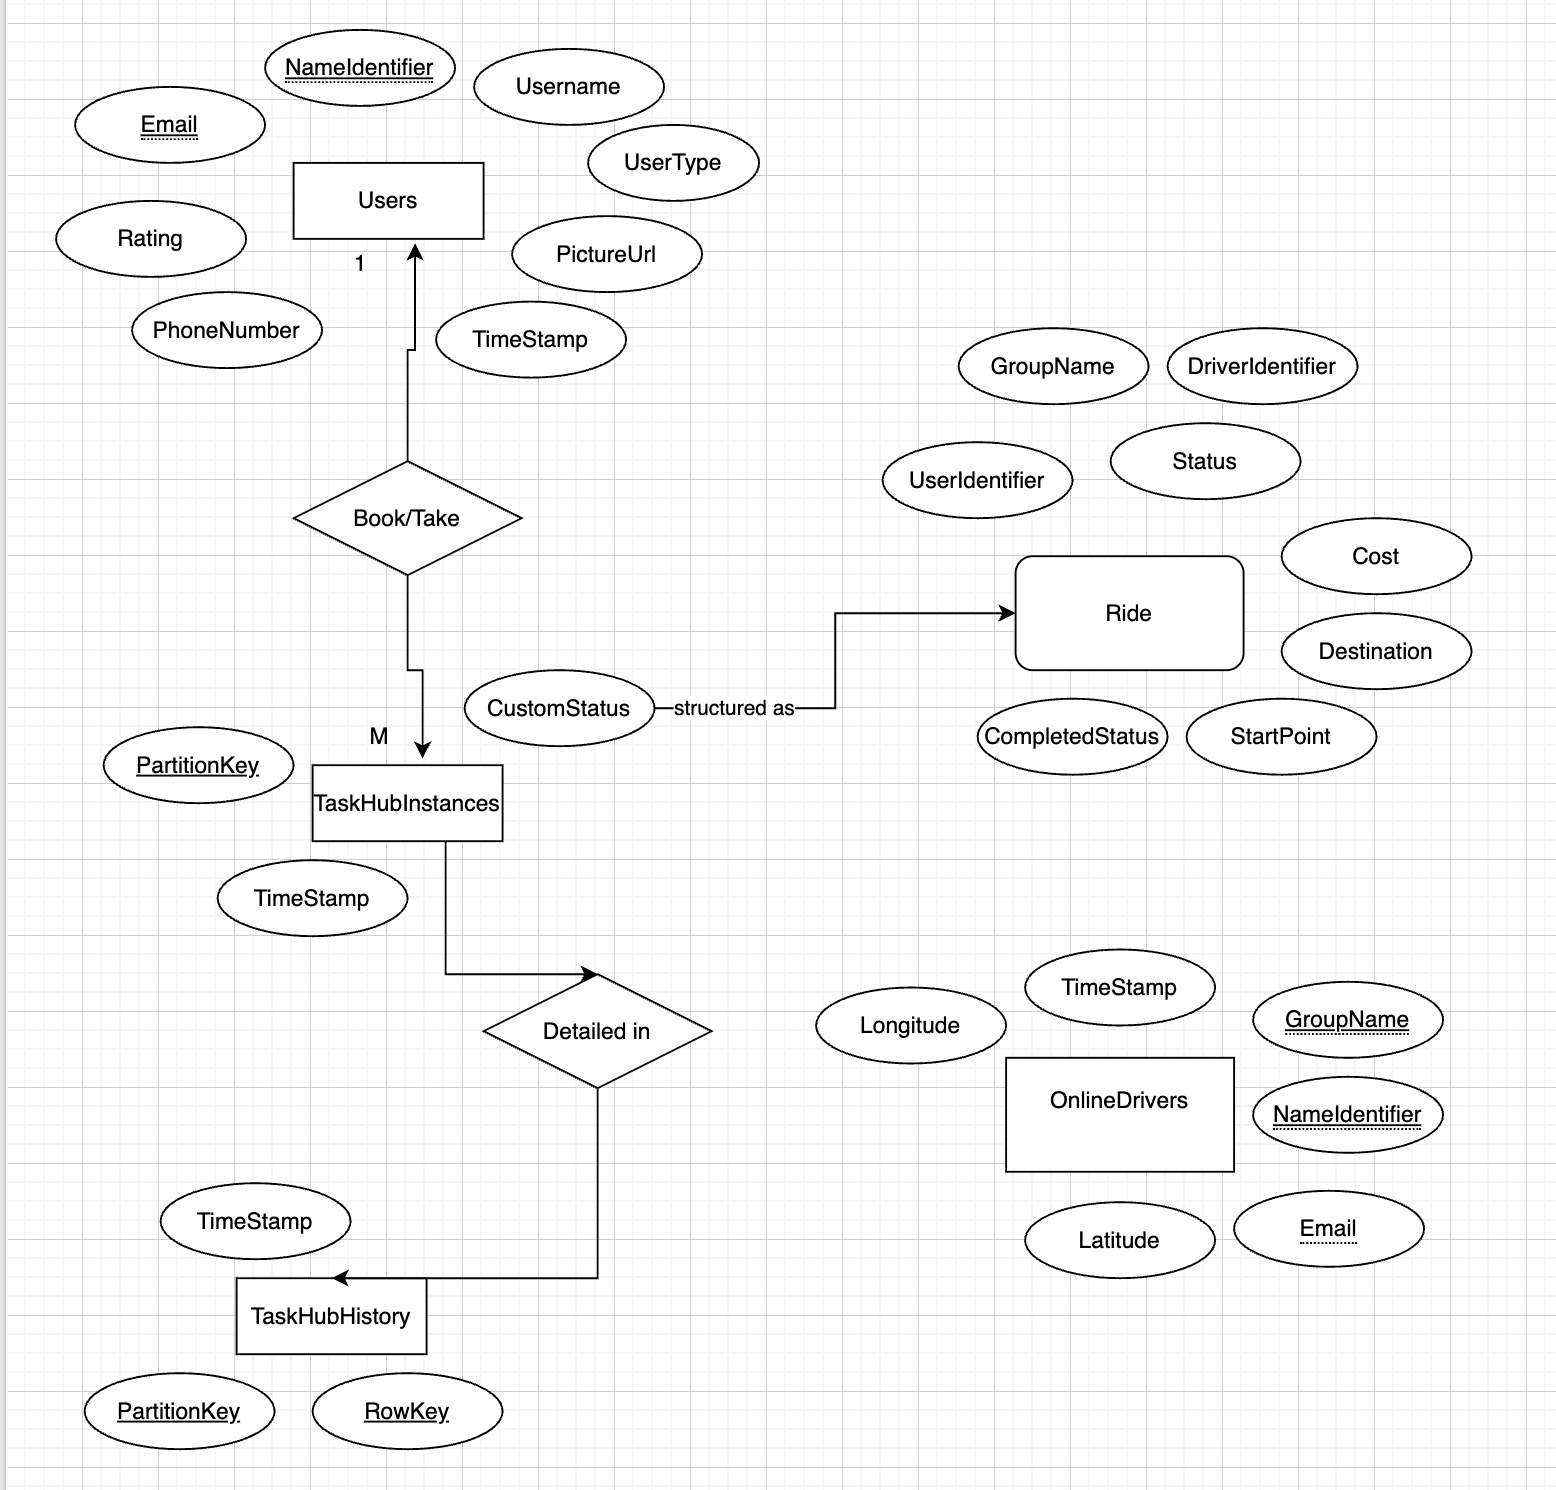
\includegraphics[width=14cm]{Assets/ER.png}
    \caption{Diagrama ER pentru baza de date.}
    \label{fig:ER}
\end{figure}

Aplicația FastRide conține trei entități, fiecare reflectând o componentă critică a
funcționalității sistemului: utilizatorii, cursele și șoferii online.

Totul pornește de la entitatea \textit{Users}, care stochează informațiile de bază ale fiecărui utilizator autentificat prin Google.
Fiecare utilizator este identificat în mod unic prin \textit{NameIdentifier} și \textit{Email}, iar alături de acesta se păstrează date precum numele (\textit{Username}), tipul de utilizator (\textit{Driver}, \textit{User} sau \textit{Admin}), ratingul acumulat de-a lungul timpului, numărul de telefon și o eventuală poză de profil (\textit{PictureUrl}).

În momentul în care un utilizator rezervă sau preia o cursă, se creează o relație între acesta și instanțele de orchestrare.
Aici intervin tabelele \textit{TaskHubInstances} și \textit{TaskHubHistory}, care reflectă intern mecanismul
de orchestrare al Azure Durable Functions. Fiecare instanță a unei funcții durabile este stocată în \textit{TaskHubInstances}, iar starea
sa (\textit{CustomStatus}) este utilizată pentru a reflecta progresul unei curse (\textit{Ride}). În paralel, \textit{TaskHubHistory} păstrează detaliile cronologice ale
execuției, istoricul exact al fiecărei acțiuni legate de instanța respectivă. Ambele entități sunt identificate prin \textit{PartitionKey}, iar
în cazul istoricului, și prin \textit{RowKey}.

Starea unei curse este gestionată de modelul \textit{Ride}, care este corelat cu Users prin câmpul \textit{UserIdentifier}, indicând clientul
care a inițiat cererea. Dacă un șofer acceptă cursa, acesta este reprezentat prin \textit{DriverIdentifier}. Fiecare cursă este
caracterizată de un status:
\begin{itemize}
    \item \textit{NewRideAvailable} - status-ul inițial al cursei
    \item \textit{GoingToUser} - momentul în care șoferul acceptă cursa și navighează către client
    \item \textit{GoingToDestination} - atunci când șoferul merge spre destinație împreună cu pasagerul
    \item \textit{Finished} - cursa este finalizată cu success
    \item \textit{Cancelled} - cursa a fost anulată
    \item \textit{None} - state-ul inițial
\end{itemize}
Mereu după ce cursa se termina, aceasta se setează pe state-ul inițial.
Pentru a face vizibil în continuare statusul final al cursei, această memorează și un \textit{CompletedStatus} :
\begin{itemize}
    \item \textit{DriverNotFound} - nu s-a găsit niciun șofer pentru a finaliza cursa
    \item \textit{PaymentRefused} - clientul a refuzat plata (disponibilă doar cu cardul)
    \item \textit{Cancelled} - cursa este anulată din orice alte motive
    \item \textit{Completed} - cursa a fost terminată cu success
\end{itemize}
În infomațiile cursei se mai regăsesc și punctul de plecare (\textit{StartPoint}),
destinația (\textit{Destination}) și costul asociat. \textit{GroupName} este folosit pentru a lega această entitate de sesiunea real-time
corespunzătoare, utilă pentru actualizări prin SignalR, astfel încât, doar șoferii din același grup cu clientul ce a inițiat cursa pot interacționa.


Pe lângă aceste entități persistente, aplicația păstrează în mod temporar o listă cu șoferii activi prin tabela \textit{OnlineDrivers}.
Fiecare șofer online este identificat prin \textit{NameIdentifier} și asociat cu \textit{GroupName}, astfel încât să poată fi notificat
în timp real dacă există cereri în zona sa. Poziția sa curentă este păstrată prin coordonatele \textit{Latitude} și \textit{Longitude},
permițând localizarea sa pe hartă.

Azure Table Storage oferă performanță, scalabilitate și costuri reduse, iar modelul este suficient
de flexibil pentru a susține dezvoltări ulterioare, cum ar fi introducerea plăților reale, recenziilor textuale
sau programării curselor în avans.

\subsection{Server-side}

Backendul aplicației este construit folosind .NET și Azure Functions, oferind o arhitectură
serverless, scalabilă și eficientă pentru gestionarea întregii logici din spatele aplicației.
Totul pornește de la faptul că aplicația este construită într-un mod în care clientul
(Blazor WebAssembly) comunică prin HTTP și SignalR cu backendul, trimițând cereri sau
ascultând în timp real anumite evenimente.

Structura proiectului Server, este cuprinsă din mai multe layere: function triggers, orchestrations,
activities, services și repositories.

\textit{Function triggers} sunt de 3 tipuri: \textit{HttpTrigger}, \textit{TimeTrigger} și \textit{SignalRTrigger}.

HttpTriggers sunt folosite pentru comunicarea cu Client-side, și sunt requesturi de tipul Get/Post și Put.
\begin{figure}[H]
    \centering
    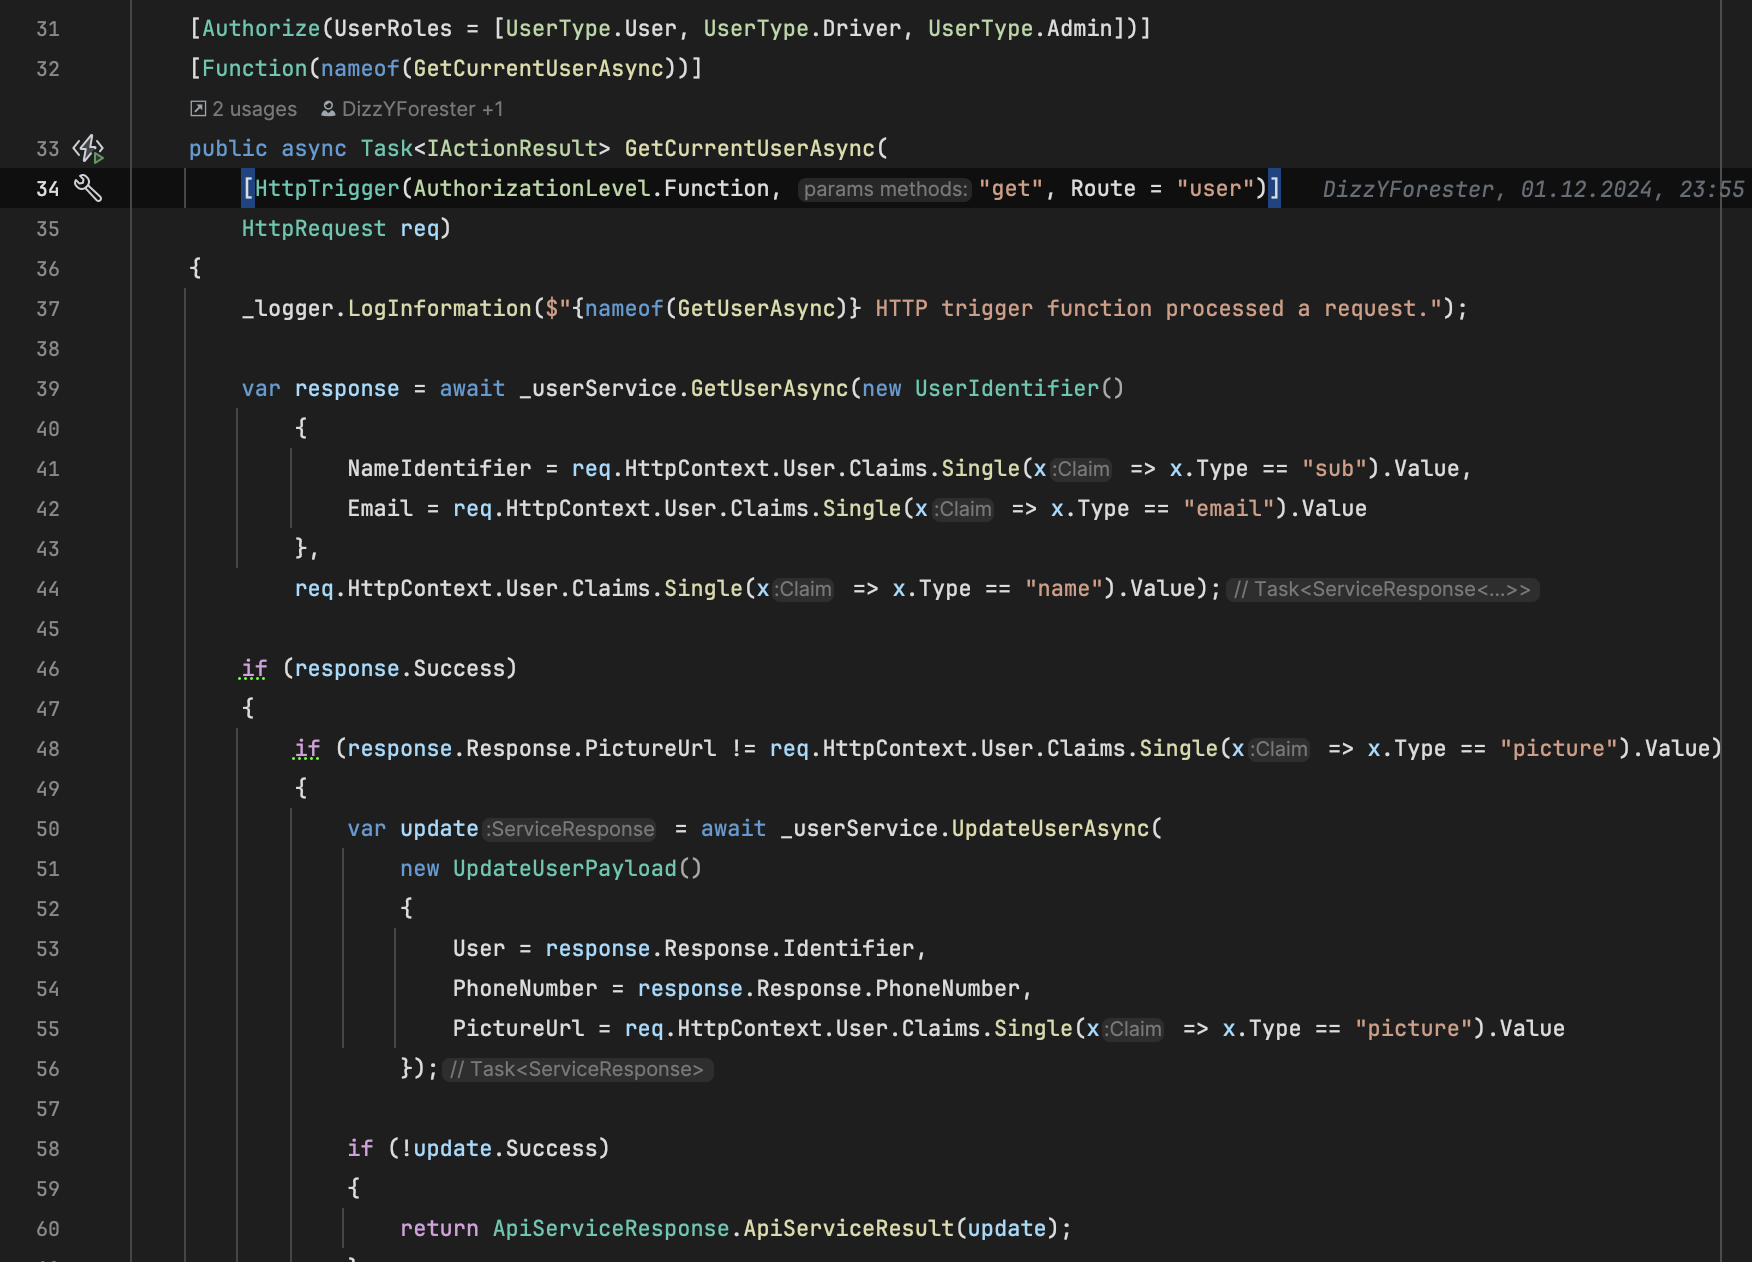
\includegraphics[width=14cm]{Assets/HttpTrigger.png}
    \caption{Exemplu de metodă GET pentru HttpTrigger function.}
    \label{fig:HttpTrigger}
\end{figure}

Aceste request-uri sunt autorizate prin Google token. Astfel s-a creat un atribut custom,
ce poate fi folosit doar pe methods, unde se pot defini o listă de \textit{roles} ce pot
accesa metoda respectivă.
Ca și request, body-ul este incapsulat în modelul \textit{HttpRequest} și poate fi deserializat
astfel:
\begin{figure}[H]
    \centering
    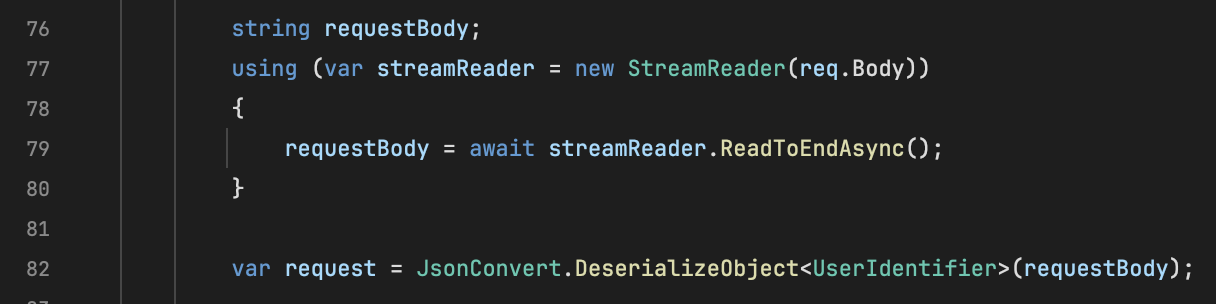
\includegraphics[width=14cm]{Assets/DeserializeRequest.png}
    \caption{Deserializarea unui request într-un tip concret (ex: \textit{UserIdentifier}).}
    \label{fig:DeserializeRequest}
\end{figure}

Ca și răspuns, toate Http functions întorc un \textit{IActionResult} ce este mapat dintr-un extension
pentru un \textit{ServiceResponse}. Acest model conține statusul request-ului, mesajul de eroare (dacă
există) și payload-ul response-ului. Toate service-urile conțin returnează un \textit{ServiceResponse}
care la fel, conține payload-ul, dacă este cu succes sau nu și mesajul de eroare împreună cu excepții.
Dacă există mesaj de eroare atunci rezultatul este un \textit{Bad Request (400)}, iar dacă există
excepție atunci se traduce ca \textit{Internal Server Error (500)}.

\begin{figure}[H]
    \centering
    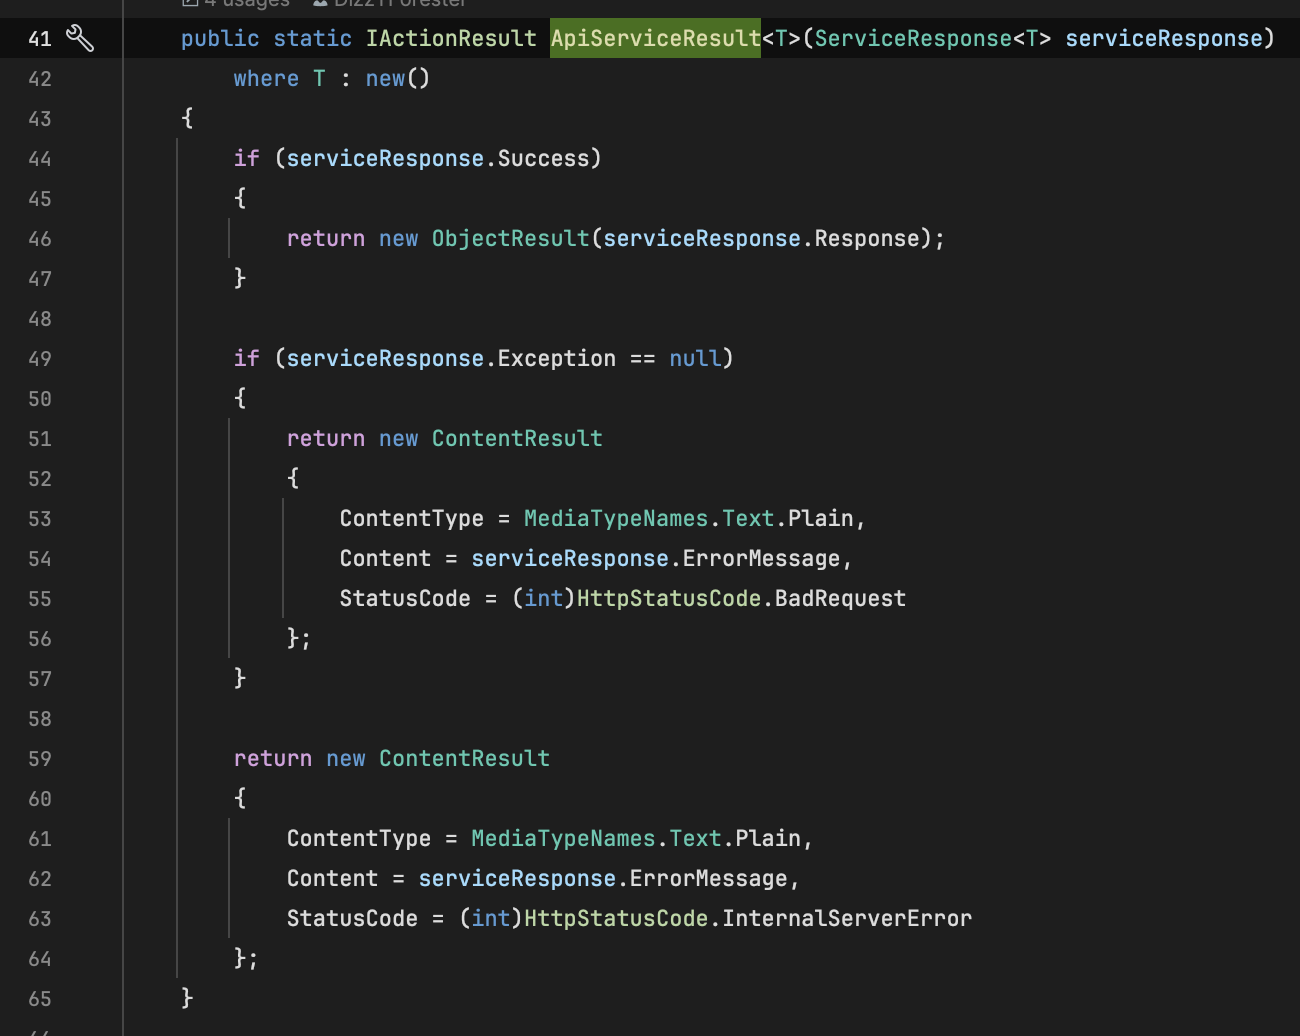
\includegraphics[width=14cm]{Assets/HttpResponse.png}
    \caption{Maparea unui \textit{ServiceResponse} la \textit{IActionResult}.}
    \label{fig:HttpResponse}
\end{figure}

Metodele HTTP disponibile pentru Client sunt:
\begin{itemize}
    \item \textit{GetCurrentUserAsync} pentru a lua informațiile despre user-ul de a inițiat requestul;
    \item \textit{GetUserAsync} pentru a lua informațiile despre un user;
    \item \textit{GetUsers}, disponibil doar pentru admini, pentru a vedea toți utilizatorii;
    \item \textit{UpdateUserAsync} pentru a actualiza un user;
    \item \textit{GetRidesByUserAsync} pentru a afișa cursele unui utilizator
\end{itemize}

Pentru a autoriza 

\subsection{Client-side}
blazor wasm si cum merge, cum apeleaza backendul
despre map si background serv§ices
\section{Comunicarea între componente}
diagrama de cum comunica aplicatia
\subsection{Autentificare și autorizare}
\subsection{Pagina admin-ului}